%!TEX TS-program = xelatex  
%!TEX encoding = UTF-8 Unicode
\documentclass[twoside, hidelinks]{book}
\hfuzz=10000pt
\hbadness=99999
\usepackage[paperheight=9.25in,
                paperwidth=7.38in,
                left=1.4in,
                right=.75in,
                top=.75in,
                bottom=1.25in,
                footskip=0.6in,
                heightrounded]{geometry}
                
\usepackage[dvipsnames]{xcolor}
\usepackage{varioref}
\usepackage{xspace}
\usepackage{fancyhdr}
\usepackage{graphicx}
\usepackage{blindtext}
\usepackage{fontspec}
\usepackage{titlesec} 
\usepackage{titletoc} 
\usepackage{listings}
\usepackage{caption}
\usepackage[unicode=true]{hyperref}


%%%  Replace english with Myanmar, tweaking varioref package 
\def\reftextfaceafter{on the \reftextvario{facing}{next} စာမျက်နှာ}%
\def\reftextfacebefore{on the \reftextvario{facing}{preceding}စာမျက်နှာ}%
\def\reftextafter{on the \reftextvario{following}{next} စာမျက်နှာ}%
\def\reftextbefore{on the \reftextvario{preceding}{previous} စာမျက်နှာ}%
\def\reftextcurrent{on \reftextvario{this}{the current} စာမျက်နှာ}%
\def\reftextfaraway#1{စာမျက်နှာ~\pageref{#1}}%
\def\reftextpagerange#1#2{on စာမျက်နှာ၂၂~\pageref{#1}--\pageref{#2}}%
\def\reftextlabelrange#1#2{\ref{#1} to~\ref{#2}}%


%%% Replace english names with Myanmar
\renewcommand{\contentsname}{မာတိကာ} 
\renewcommand{\chaptername}{}
\renewcommand{\figurename}{ပုံ}


%%% definition of Apple colors
\definecolor{iron}{HTML}{5E5E5E}
\definecolor{steel}{HTML}{797979}
\definecolor{tungsten}{HTML}{424242}
\definecolor{lead}{HTML}{212121}
\definecolor{steelblue}{HTML}{36648B}


%%% Page style related stuff
\fancyhf{}
\fancyhead[LE]{\color{steelblue}\bfseries\mmpdk\nouppercase{\leftmark}}
\fancyhead[RO]{\color{steelblue}\bfseries\mmpdk\nouppercase{\rightmark}}
\fancyfoot[LE,RO]{\thepage}
\pagestyle{fancy}
\setlength{\headsep}{15pt}
\setlength{\headheight}{30pt}% ...at least 51.60004pt
\renewcommand\headrule{
\begin{minipage}
    {1\textwidth}
    \color{MidnightBlue}\hrule width \hsize \kern 1mm 
    \color{MidnightBlue}\hrule width \hsize height 2pt 
\end{minipage}}%


%%% Font related tweaks
\defaultfontfeatures{Script=Myanmar,Mapping=tex-text} 
\fontspec[Script=Myanmar, BoldFont={Padauk Book Bold}, ]{Padauk Book}
\setmainfont[UprightFont={Padauk Book},
                BoldFont={Padauk Book Bold},
                ItalicFont={Padauk Book},
                BoldItalicFont={Padauk Book Bold},
                SmallCapsFont={Padauk Book},
                SlantedFont={Padauk Book}]{Padauk Book}
                [Renderer=Harfbuzz,Script=Myanmar]


%%% Define fonts english font to be used in between Myanmar text               
% Helvetica Neue, Geneva, Tahoma
% Font for normal english words and program code related words to be used in paragraph
%\newfontfamily\myparaen[Color=tungsten, Scale=MatchLowercase]{Verdana}
%\newfontfamily\mycode[Color=lead, Scale=1]{Ubuntu Mono}

%\DeclareTextFontCommand{\myen}{\myparaen}
%\DeclareTextFontCommand{\txtmycode}{\mycode}

\newcommand{\mmem}[1]{\textbf{\color{blue}#1}}

\newcommand{\mmpdk}       {\fontspec[Script=Myanmar,Scale=1]{Myanmar Tagu}\selectfont}

%%% Switching to type writer font and sans serif font in paragraph
% Make sure to set the color to match the main font color
\newcommand{\mycodetmp}   {\fontspec[Scale=1]{Ubuntu Mono}\selectfont}
\newcommand{\myentmp}     {\fontspec[Scale=1,Scale=MatchLowercase]{Verdana}\selectfont}
% Limiting the scope of the selected font
\newcommand{\mycode}   [1]{{\mycodetmp{#1}}}
\newcommand{\myen}   [1]{{\myentmp{#1}}}

%%% With \XeTeXinterwordspaceshaping=2, \color or \textcolor doesn't work 
% This is a workaround to color text 
\newcommand{\myemcodetmp}   {\fontspec[Scale=1, Color=red]{Ubuntu Mono}\selectfont}
\newcommand{\myementmp}     {\fontspec[Scale=1,Scale=MatchLowercase, Color=red]{Verdana}\selectfont}
\newcommand{\myemmmtmp}     {\fontspec[Scale=1,Scale=MatchLowercase, Color=red]{Padauk Book}\selectfont}
% Limiting the scope of the selected font
\newcommand{\myemcode}   [1]{{\myemcodetmp{#1}}}
\newcommand{\myemen}   [1]{{\myementmp{#1}}}
\newcommand{\myemmm}   [1]{{\myemmmtmp{#1}}}

\newcommand{\mydefcodetmp}   {\fontspec[Scale=1, Color=MidnightBlue]{Ubuntu Mono}\selectfont}
\newcommand{\mydefentmp}     {\fontspec[Scale=1,Scale=MatchLowercase, Color=MidnightBlue]{Verdana}\selectfont}
\newcommand{\mydefmmtmp}     {\fontspec[Scale=1,Scale=MatchLowercase, Color=MidnightBlue]{Padauk Book}\selectfont}
% Limiting the scope of the selected font
\newcommand{\mydefcode}   [1]{{\mydefcodetmp{#1}}}
\newcommand{\mydefen}   [1]{{\mydefentmp{#1}}}
\newcommand{\mydefmm}   [1]{{\mydefmmtmp{#1}}}


%%% Switching to type writer font and sans serif font in titles and caption
% Make sure not to set the color. Color should be applied later at the respective
% formatting applied to titles, caption, headers etc.,
\newcommand{\myttlcodetmp}   {\fontspec[Scale=1]{Ubuntu Mono}\selectfont}
\newcommand{\myttlentmp}   {\fontspec[Scale=1,Scale=MatchLowercase]{Verdana}\selectfont}
% Limiting the scope of the selected font
\newcommand{\myttlcode}   [1]{{\myttlcodetmp{#1}}}
\newcommand{\myttlen}   [1]{{\myttlentmp{#1}}}

%%% Changes the spacing for everything in the document, including footnotes and tables 
\renewcommand{\baselinestretch}{1.35} 


%%% Auto numbering in Myanmar %%%
%This macro is to produce myanmar numbering by adopting the thai numbering method
\makeatletter  
\def\@mmnum#1{\expandafter\@@mmnum\number#1\@nil}  
\def\@@mmnum#1{%  
  \ifx#1\@nil  
  \else  
  \char\numexpr#1+"1040\relax  
  \expandafter\@@mmnum\fi  
}  
\renewcommand\@arabic{\@mmnum} % to reset number in \arabic to \mmnum 
\makeatother 


%%% Formatting part, chapter, section, subsection, subsubsection heading and table of contents
%%% and caption
% For caption
\DeclareCaptionFont{captionfont}{\color{iron}\bfseries\fontspec[Script=Myanmar,Scale=0.9]{Pyidaungsu Bold}\selectfont}
\captionsetup{font=captionfont}
% For table of contents
\contentsmargin[1cm]{0cm}
\titlecontents{chapter}[0em]{\color{steelblue}\large\bfseries\mmpdk}
{\thecontentslabel\enspace}
{\hspace{1.05em}}
{ \hfill\contentspage}[\vskip 6pt]

\titlecontents{section}[1em]{\color{steelblue}\normalsize\bfseries\mmpdk}
{\thecontentslabel\enspace}
{}
{\titlerule*[1pc]{.}\quad\contentspage}[\vskip 4pt]

\titlecontents{subsection}[2.7em]{\color{steelblue}\normalfont\bfseries\mmpdk}
{\thecontentslabel\enspace}
{}
{\titlerule*[1pc]{.}\quad\contentspage}[\vskip 3pt]

% For titles and their name in headers
\titleformat{\section}[block] 
{\color{MidnightBlue}\normalfont\large\bfseries\mmpdk }{{\color{MidnightBlue}\large\thesection}}{1em}{}

\titleformat{\subsection}[block] 
{\color{MidnightBlue}\normalsize \mmpdk}{{\color{MidnightBlue}\normalsize\thesubsection}}{1em}{}

\titleformat{\subsubsection}[block] 
{\color{MidnightBlue}\normalsize\mmpdk }{{\color{MidnightBlue}\normalsize\thesubsubsection}}{1em}{}

\titleformat{\chapter}[display] 
    {\color{MidnightBlue}\normalfont\Huge\bfseries\mmpdk }{\color{MidnightBlue}{\Huge\mmpdk\thechapter}}{1ex}
    {\filright} 

\titleformat{\part}[display] 
{\filcenter\LARGE\mmpdk}{{\large\partname\; \thepart}}{1em}{\thispagestyle{empty}}

%%% Code listing related
\newfontface\pgcode[Scale=0.9, BoldFont={Ubuntu Mono Bold}]{Ubuntu Mono}
\lstset{
  language     = Java,
  basicstyle   = \pgcode,
  commentstyle = \color{gray},
  keywordstyle = \color{darkgray}\textbf,
  stringstyle  = \color{green!70!black},
  stringstyle  = \color{red},
  columns      = fullflexible,
  numbers      = left,
  numberstyle  = \scriptsize\sffamily\color{gray},
  caption      = A hello world program in Java,
  showstringspaces = false,
}

%%% Custom utility commands
\newcommand*\cleartoleftpage{%
  \clearpage
  \ifodd\value{page}\hbox{}\newpage\fi
}

\newcommand{\todef}[1]{\textbf{#1}}
\newcommand{\toem}[1]{\textbf{#1}}

\newcommand{\Fig}{ပုံ\xspace}
\newcommand{\enprogramming}{ပရိုဂရမ်းမင်း{\myen{(programming)}}}
\newcommand{\mmprogramming}{ပရိုဂရမ်းမင်း}
\newcommand{\enprogram}{ပရိုဂရမ်{\myen{(program)}}}
\newcommand{\mmprogram}{ပရိုဂရမ်}
\newcommand{\encommand}{ကွန်မန်း{\myen{(command)}}}
\newcommand{\mmcommand}{ကွန်မန်း}
\newcommand{\encorner}{ကွန်နာ{\myen{(corner)}}}
\newcommand{\mmcorner}{ကွန်နာ}
\newcommand{\enbeeper}{ဘိပါ{\myen{(beeper)}}}
\newcommand{\mmbeeper}{ဘိပါ}
\newcommand{\enprogramCode}{ပရိုဂရမ်ကုဒ်{\myen{(program code)}}}
\newcommand{\mmprogramCode}{ပရိုဂရမ်ကုဒ်}
\newcommand{\enprogrammingLanguageDef}{ပရိုဂရမ်ရေးရန် အသုံးပြုသည့် ဘာသာစကား{\myen{(programming language)}}}
\newcommand{\enprogrammingLanguage}{{\myen{programming language}}\xspace}
\newcommand{\encontrolFlowStatement}{{\myen{control flow statement}}\xspace}

\newcommand{\enprog}{\enprogramming}



\title{\mmpdk အခြေခံ ပရိုဂရမ် ရေးနည်း } 
\author{ပြည်စိုး} 
\date{၀၅/၀၅/၂၀၂၂}

\begin{document}

\setcounter{secnumdepth}{3} % counter for susubsection
\setcounter{tocdepth}{3} % to view susubsection in toc

\frontmatter
\maketitle
\tableofcontents
\cleardoublepage

\mainmatter
\chapter{စက်ရုပ်ကားရဲလ် {\myttlcode{for}} Programming with Karel the Robot}
\XeTeXlinebreaklocale "my_MM"  %Myanmar line and character breaks
\XeTeXinterwordspaceshaping=2
\begin{sloppypar}
\enprogramming\ ဆိုတာဘာလဲ။ ဒါကိုဖြေဖို့ စာတွေအများကြီးရေးပြီး ရှင်းပြလို့ရပေမယ့် အများကြီးသိပ်မပြောပဲ လက်တွေ့ \enprogram လေးတွေ စရေးကြည့်ပြီးမှ \mmprogramming ဆိုတာ ဘာလဲ ပြောပြလိုက်ရင် ပိုပြီးနားလည်ရလွယ်တယ်။ ဒါ့ကြောင့် စက်ရုပ်ကားရဲလ်\txtmyparaen{(Karel the Robot)}ကို အလုပ်တွေ လုပ်ခိုင်းဖို့ \mmprogram လေးတွေ  အရင်ဆုံး ရေးကြည့်ကြမယ်။

စက်ရုပ်ကားရဲလ်က အခြေခံအားဖြင့် \txtmycode{move, turnLeft, putBeeper, pickBeeper} ဆိုတဲ့ ကွန်မန်း\txtmyparaen{(command)} လေးခုကို နားလည်တယ်။ \txtmycode{move} ကွန်မန်းက သူရပ်နေတဲ့ ကွန်နာ\txtmyparaen{(corner)}ကနေ ရှေ့တည့်တည့် ကပ်ရပ် ကွန်နာဆီကို ရွှေ့ခိုင်းတာ။ \Fig \vref*{fig:name} မှာပြထားတဲ့ ကြက်ခြေခတ်လေးတွေကို ကွန်နာလို့ခေါ်တယ်။ 

\begin{figure}[!b]
    \centering\caption{ကားရဲလ်၏ {\myttlcode{for}} ကမ္ဘာ}\label{fig:name}
    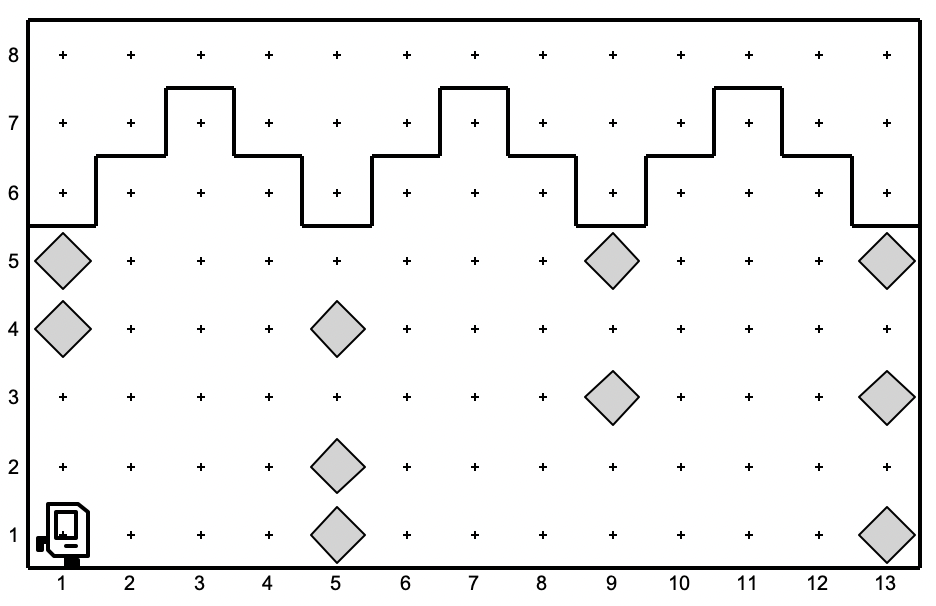
\includegraphics[width=4in]{ch01/ch01}
\end{figure}


\txtmycode{turnLeft} ကွန်မန်းကတော့ ဘယ်ဘက်လှည့်ခိုင်းတာ။ ကားရဲမျက်နှာမူရာ အရပ်မျက်နှာ တစ်ခုချင်းစီအတွက် \txtmycode{turnLeft} ကွန်မန်းပေးလိုက်တဲ့ အခါမှာ ဘယ်အရပ်ကိုလှည့်သွားမလဲ ပုံမှာတွေ့နိုင်တယ်။

ကားရဲလ်ကို \txtmycode{putBeeper} ကွန်မန်းပေးလိုက်ရင်တော့ ကားရဲလ်က သူရှိနေတဲ့ ကွန်နာမှာ ဘိပါ\txtmyparaen{(beeper)} လို့ခေါ်တဲ့ အတုံးလေး တစ်ခုချထားလိမ့်မယ်။ ဒီကွန်မန်း မပေးရသေးခင်နဲ့ ပေးပြီးအခြေအနေကို ပုံမှာယှဉ်ပြထားတယ်။ ကွန်မန်းပေးပြီးသွားတဲ့အခါ စိန်တုံးပုံစံ ဘိပါတုံးလေး ရှိနေတာ တွေ့ရမယ်။ 

\txtmycode{pickBeeper} ကွန်မန်းက ဘိပါကောက်ခိုင်းတာပါ။ ကားရဲလ်ရောက်နေတဲ့ ကွန်နာမှာ ဘိပါရှိရင် ဒီကွန်မန်းနဲ့ ကောက်ခိုင်းလို့ရတယ်။ ကွန်နာတစ်ခုမှာ ဘိပါတစ်ခုမက ရှိနိုင်တယ်။ တစ်ခုမှ မရှိတာလဲ ဖြစ်နိုင်တယ်။ ပုံမှာဆိုရင် ကွန်နာတစ်ခုမှာပဲ ဘိပါရှိနေပြီး ကျန်တဲ့ ကွန်နာတွေမှာက ဘိပါမရှိပါဘူး။

ပရိုဂရမ်းမင်း\txtmyparaen{(programming)} ဆိုတာဘာလဲ။ ဒါကိုဖြေဖို့ စာတွေအများကြီးရေးပြီး ရှင်းပြလို့ရသလို အများကြီးသိပ်မပြောပဲ လက်တွေ့ \txtmyparaen{program} လေးတွေစရေးကြည့်ပြီးမှ ပရိုဂရမ်းမင်းဆိုတာ ဘာလဲ ပြောပြလိုက်ရင် ပိုပြီးနားလည်ရလွယ်တယ်။ ဒါ့ကြောင့် စက်ရုပ်ကားရဲလ်\txtmyparaen{(Karel the Robot)}ကို အလုပ်တွေ လုပ်ခိုင်းဖို့ ပရိုဂရမ်\txtmyparaen{(program)} လေးတွေ အရင်ဆုံး ရေးကြည့်ကြမယ်။

စက်ရုပ်ကားရဲလ်က အခြေခံအားဖြင့် \txtmycode{move, turnLeft, putBeeper, pickBeeper} ဆိုတဲ့ ကွန်မန်း\txtmyparaen{(command)} လေးခုကို နားလည်တယ်။ \txtmycode{move} ကွန်မန်းက သူရပ်နေတဲ့ ကွန်နာ\txtmyparaen{(corner)}ကနေ ရှေ့တည့်တည့် ကပ်ရပ် ကွန်နာဆီကို ရွှေ့ခိုင်းတာ။ ပုံမှာပြထားတဲ့ ကြက်ခြေခတ်လေးတွေကို ကွန်နာလို့ခေါ်တယ်။ 

\txtmycode{turnLeft} ကွန်မန်းကတော့ ဘယ်ဘက်လှည့်ခိုင်းတာ။ ကားရဲမျက်နှာမူရာ အရပ်မျက်နှာ တစ်ခုချင်းစီအတွက် \txtmycode{turnLeft} ကွန်မန်းပေးလိုက်တဲ့ အခါမှာ ဘယ်အရပ်ကိုလှည့်သွားမလဲ ပုံမှာတွေ့နိုင်တယ်။

ကားရဲလ်ကို \txtmycode{putBeeper} ကွန်မန်းပေးလိုက်ရင်တော့ ကားရဲလ်က သူရှိနေတဲ့ ကွန်နာမှာ ဘိပါ\txtmyparaen{(beeper)} လို့ခေါ်တဲ့ အတုံးလေး တစ်ခုချထားလိမ့်မယ်။ ဒီကွန်မန်း မပေးရသေးခင်နဲ့ ပေးပြီးအခြေအနေကို ပုံမှာယှဉ်ပြထားတယ်။ ကွန်မန်းပေးပြီးသွားတဲ့အခါ စိန်တုံးပုံစံ ဘိပါတုံးလေး ရှိနေတာ တွေ့ရမယ်။ 

\txtmycode{pickBeeper} ကွန်မန်းက ဘိပါကောက်ခိုင်းတာပါ။ ကားရဲလ်ရောက်နေတဲ့ ကွန်နာမှာ ဘိပါရှိရင် ဒီကွန်မန်းနဲ့ ကောက်ခိုင်းလို့ရတယ်။ ကွန်နာတစ်ခုမှာ ဘိပါတစ်ခုမက ရှိနိုင်တယ်။ တစ်ခုမှ မရှိတာလဲ ဖြစ်နိုင်တယ်။ ပုံမှာဆိုရင် ကွန်နာတစ်ခုမှာပဲ ဘိပါရှိနေပြီး ကျန်တဲ့ ကွန်နာတွေမှာက ဘိပါမရှိပါဘူး။ \vref*{fig:name} မှာပြထားတဲ့ ကြက်ခြေခတ်လေးတွေကို ကွန်နာလို့ခေါ်တယ်။ 

ပရိုဂရမ်းမင်း\txtmyparaen{(programming)} ဆိုတာဘာလဲ။ ဒါကိုဖြေဖို့ စာတွေအများကြီးရေးပြီး ရှင်းပြလို့ရသလို အများကြီးသိပ်မပြောပဲ လက်တွေ့ \txtmyparaen{program} လေးတွေစရေးကြည့်ပြီးမှ ပရိုဂရမ်းမင်းဆိုတာ ဘာလဲ ပြောပြလိုက်ရင် ပိုပြီးနားလည်ရလွယ်တယ်။ ဒါ့ကြောင့် စက်ရုပ်ကားရဲလ်\txtmyparaen{(Karel the Robot)}ကို အလုပ်တွေ လုပ်ခိုင်းဖို့ ပရိုဂရမ်\txtmyparaen{(program)} လေးတွေ အရင်ဆုံး ရေးကြည့်ကြမယ်။

စက်ရုပ်ကားရဲလ်က အခြေခံအားဖြင့် \txtmycode{move, turnLeft, putBeeper, pickBeeper} ဆိုတဲ့ ကွန်မန်း\txtmyparaen{(command)} လေးခုကို နားလည်တယ်။ \txtmycode{move} ကွန်မန်းက သူရပ်နေတဲ့ ကွန်နာ\txtmyparaen{(corner)}ကနေ ရှေ့တည့်တည့် ကပ်ရပ် ကွန်နာဆီကို ရွှေ့ခိုင်းတာ။ ပုံမှာပြထားတဲ့ ကြက်ခြေခတ်လေးတွေကို ကွန်နာလို့ခေါ်တယ်။ 

\txtmycode{turnLeft} ကွန်မန်းကတော့ ဘယ်ဘက်လှည့်ခိုင်းတာ။ ကားရဲမျက်နှာမူရာ အရပ်မျက်နှာ တစ်ခုချင်းစီအတွက် \txtmycode{turnLeft} ကွန်မန်းပေးလိုက်တဲ့ အခါမှာ ဘယ်အရပ်ကိုလှည့်သွားမလဲ ပုံမှာတွေ့နိုင်တယ်။

ကားရဲလ်ကို \txtmycode{putBeeper} ကွန်မန်းပေးလိုက်ရင်တော့ ကားရဲလ်က သူရှိနေတဲ့ ကွန်နာမှာ ဘိပါ\txtmyparaen{(beeper)} လို့ခေါ်တဲ့ အတုံးလေး တစ်ခုချထားလိမ့်မယ်။ ဒီကွန်မန်း မပေးရသေးခင်နဲ့ ပေးပြီးအခြေအနေကို ပုံမှာယှဉ်ပြထားတယ်။ ကွန်မန်းပေးပြီးသွားတဲ့အခါ စိန်တုံးပုံစံ ဘိပါတုံးလေး ရှိနေတာ တွေ့ရမယ်။ 

\txtmycode{pickBeeper} ကွန်မန်းက ဘိပါကောက်ခိုင်းတာပါ။ ကားရဲလ်ရောက်နေတဲ့ ကွန်နာမှာ ဘိပါရှိရင် ဒီကွန်မန်းနဲ့ ကောက်ခိုင်းလို့ရတယ်။ ကွန်နာတစ်ခုမှာ ဘိပါတစ်ခုမက ရှိနိုင်တယ်။ တစ်ခုမှ မရှိတာလဲ ဖြစ်နိုင်တယ်။ ပုံမှာဆိုရင် ကွန်နာတစ်ခုမှာပဲ ဘိပါရှိနေပြီး ကျန်တဲ့ ကွန်နာတွေမှာက ဘိပါမရှိပါဘူး။ \Fig\vref*{fig:name} မှာပြထားတဲ့ ကြက်ခြေခတ်လေးတွေကို ကွန်နာလို့ခေါ်တယ်။ 

\end{sloppypar}

\chapter{Control Flow}
\XeTeXlinebreaklocale "my_MM"  %Myanmar line and character breaks
\XeTeXinterwordspaceshaping=2
\begin{sloppypar}
\color{tungsten}
ကားရဲလ်ကို ရှေ့ကို ၂၅ လှမ်း ရွှေ့ခိုင်းချင်တယ်။ \mycode{move(); move(); move(); ...move();} ၂၅ ခါ ရေးလို့‌တော့ရတာပေါ့။ ဒါပေမယ့် စာရိုက်ရတာ အချိန်လည်းကုန် လက်လဲညောင်း ဖြစ်မယ်။ {\mycode{move();}} ကို ၂၅ ကြိမ် ကျော့ပေးပါလို့ ခိုင်းလို့ရရင် ပိုမကောင်းဘူးလား။ 

ကားရဲလ်ရဲ့ ရှေ့တည့်တည့် ခပ်လှမ်းလှမ်းမှာ နံရံတစ်ခုရှိနေမယ်။ ဘယ်လောက်ဝေးလဲ မသိဘူးဆိုပါစို့။ ကားရဲလ်ကို နံရံဆီရောက်အောင် သွားခိုင်းချင်တယ်။ နံရံက ဘယ်လောက်ဝေးလဲ မသိတော့ {\mycode{move}} ကို ဘယ်နှစ်ကြိမ် ကျော့ခိုင်းရမလဲ မသိနိုင်ဘူး။ ရှေ့မှာရှင်းနေသေးသ၍ \mycode{move} ပါလို့သာ ခိုင်းလို့ရမယ်ဆိုရင် တော်တော်လေး အဆင်ပြေပြီ။  

အခြေအနေတစ်ခု မှန်တော့မှပဲ \mmcommand တွေကို လုပ်ဆောင်စေချင်တာမျိုးလဲ ရှိတယ်။ အဲဒီ အခြေနေနဲ့ မကိုက်ညီဘူး (တနည်းအားဖြင့် အခြေအနေက မှားနေခဲ့ရင်) \mmcommand တွေကို မလုပ်ဆောင်ပဲ ကျော်သွားစေချင်တယ်။ ရှေ့မှာပြောခဲ့တဲ့ နံရံအောက််ခြေမှာ \mmbeeper တစ်ခု ရှိနေနိုင်တယ်၊ ရှိချင်မှလည်း ရှိမယ်ဆိုပါစို့။ \mmbeeper ရှိနေခဲ့ရင် နံရံ အခြားတဘက်မှာ \mmbeeper ကို ထားခိုင်းချင်တယ်။  ဒါဆိုရင် \mmbeeper ရှိနေမှပဲ အခြားတဘက်ကို ရွှေ့ခိုင်းဖို့ လိုအပ်တဲ့ \mmcommand တွေကို လုပ်ဆောင်စေချင်တယ်။ \mmbeeper မရှိဘူးဆိုရင် အဲဒီ \mmcommand တွေကို မလုပ်ဆောင်စေချင်ဘူး။  

 နောက်ထပ်တစ်မျိုးက အခြေအနေတစ်ခု မှန်ခဲ့ရင် လုပ်ဆောင်စေချင်တဲ့ \mmcommand တွေနဲ့ မှားခဲ့ရင်‌ လုပ်ဆောင်စေချင်တဲ့ \mmcommand ‌တွေကို မတူပဲဖြစ်နေတာမျိုးပါ။ တနည်းအားဖြင့် အခြေအနေပေါ် မူတည်ပြီး ခိုင်းရမယ့် အလုပ်ကမတူဘူး။ \mmbeeper ရှိခဲ့ရင် နံရံရဲ့ အခြားဘက်ကိုရွှေ့ခိုင်းချင်တယ်၊ မရှိခဲ့ရင်တော့ လာလမ်းအတိုင်း ပြန်လာစေချင်တယ် ဆိုပါစို့။ ဒါဆိုရင် \mmbeeper ရှိခြင်း၊ မရှိခြင်းပေါ် မူတည်ပြီး လုပ်ဆောင်ရမယ့် \mmcommand တွေက မတူဘူး။ 


 အသုံးပြုရတဲ့ \toem{\myemen{control flow statements} \myemmm{များတွင်} \myemcode{for, while, if, if else} \myemmm{တို့ပါဝင်သည်။} } \color{tungsten} တွေကို  ဒီအခန်းမှာ ‌လေ့လာကြမယ်။ ကမ္ဘာ့

 အသုံးပြုရတဲ့ \todef{\mydefen{control flow statements} \mydefmm{များတွင်} \mydefcode{for, while, if, if else} \mydefmm{တို့ပါဝင်သည်။} } \color{tungsten} တွေကို  ဒီအခန်းမှာ ‌လေ့လာကြမယ်။ ကမ္ဘာ့

 

 \section{{\myttlcode{for}} loop}

 \section{{\myttlcode{while}} loop}

 \section{{\myttlcode{if}} and {\myttlcode{if else}} statements}

 \section{Nested structures}




 % \mmcommand တွေကို ထပ်ခါထပ်ခါ ပြန်ကျော့ခိုင်းဖို့ လိုအပ်လေ့ရှိတယ်။ 
 %\mmprogram တွေရေးတဲ့အခါမှာ \mmcommand တွေကို အခြေအနေတစ်ခု မှန်နေသ၍ ပြန်ကျော့ပြီးလုပ်ဆောင်ခိုင်းဖို့ လိုအပ်လေ့ရှိတယ်။
 %
\end{sloppypar}

\chapter{\myenchttl{Program Design - Solving More Complex Programs} ပရိုဂရမ် ဒီဇိုင်း}
\XeTeXlinebreaklocale "my_MM"  %Myanmar line and character breaks
\XeTeXinterwordspaceshaping=2
\begin{sloppypar}


    sdfd
  asasa

\end{sloppypar}




\end{document}